\section {Choix effectués}

\subsection{Algorithme de référence}

Un premier algorithme naïf a été écrit. Il s'agit d'une simple double
boucles qui, pour chaque case, fait écrouler le tas de sable sur les
quatre cases voisines.  Nous utilisons cette algorithme comme
référence pour vérifier que les algorithmes optimisés ou parallèles
donnent des résultats corrects. Il s'agit de la méthode
\texttt{compute\_naïve} (algorithme~\ref{algo:naif}).
\medskip

\subsection{Optimiser l'utilisation du cache}
\label{sec:cache}

Nous allouons un tableau de taille $DIM*DIM$ et pour nous y faciliter les
accès, on alloue un deuxième tableau de taille $DIM$ dont chaque case
pointe sur une ligne différente (de taille $DIM$) du premier tableau.

Dans le cache L1 (32 KB), on peut faire rentrer
$32*1024/sizeof(unsigned)/DIM$ lignes de la matrice soit 64 lignes
pour la matrice de dimension 128 et 16 lignes pour celle de dimension
512. Il est donc naturel de parcourir la matrice ligne par ligne.

\subsection{Algorithmes séquentiels}

\subsubsection{Division euclidienne}

Une première optimisation simple consiste à effectuer des divisions
euclidiennes pour faire ébouler un tas de sable d'un seul coup sur les
cases voisines. L'avantage est que si un case contient un grand nombre
de grains de sable, on va pouvoir la vider en une
opération. Seulement, à l'itération suivante, un huitième des grains
de sable envoyés chez les voisins reviennent sur la case de départ.
Il s'agit de la méthode \texttt{compute\_eucl} (algorithme~).
\medskip

\subsubsection{Prédiction de branchement}

Une autre optimisation consiste à mieux utiliser la prédiction de
branchement du processeur. À chaque itération et pour chaque case, on
vérifie si la case dépasse une certaine valeur (la taille maximale
d'un tas de sable avant éboulement). Or, comme d'une case à l'autre le
contenu peut être radicalement différent, on peut peut pas
statistiquement prédire si nous allons effectuer un changement (un
éboulement) ou non. La prédiction de branchement n'est donc pas
efficace ici.
\medskip

Il faut alors effectuer toujours les mêmes opérations, qu'il y ait
un changement ou non.
\medskip

% 5 à 7 fois plus vite en seq, 2 fois plus vite en para

\subsubsection{Diminuer les accès en écriture}

Une autre approche que l'éboulement du tas de sable sur les cases
voisines consistes à consulter le hauteur du tas de chacun de des
voisins d'une case. En fonction de ces quatre hauteurs, on met à jour
la valeur de la case, en faisant écrouler les tas de sables voisins
sur la case, mais sans modifier le contenu des cases voisines. Avec
cette approche, à chaque itération et pour chaque case, on effectue 5
accès lecture et un accès écriture contre 5 accès lecture et écriture
pour l'autre approche. Il s'agit de la méthode
\texttt{compute\_eucl\_swap} (algorithme~TODO).
\medskip

L'inconvénient de cette approche est qu'on ne peut pas lire et écrire
dans la même matrice sinon les résultats seraient faux. Ainsi, on
dispose d'une matrice d'écriture et d'une matrice de lecture. Pendant
qu'on lit la matrice de lecture, on écrit sur une matrice
auxiliaire. Ensuite, après une itération, on échange la matrice de
lecture et d'écriture.
\medskip

Nous pouvons avec cette méthode facilement effectuer le même
traitement qu'il faille ébouler une case ou non. Ainsi, nous pouvons
éviter les prédictions de branchement incorrects.
\bigskip

Nous avons essayé d'autres approches comme la détection des zones
stables, \texttt{compute\_\-eucl\_\-chunk}, ou l'utilisation
d'opérations vectorielles pour tenter de traiter plusieurs cases d'un
seul coup, \texttt{compute\_\-eucl\_\-vector}.
\medskip

\subsection{Algorithmes multi-threads}

\subsubsection{Paralléliser une itération de l'algorithme}

Une première solution multi-threads a été réalisée à l'aide
d'OpenMP. Il s'agit de la méthode \texttt{compute\_omp}.
\medskip

Nous avons déjà vu section~\ref{sec:cache} que pacourir la matrice
ligne par ligne est la façon qui permet d'utiliser au mieux le cache.4

Pour la plupart de nos solutions multi-threads, nous répartissons le
traitement de chaque ligne de la matrice sur un ensemble de
threads. Un thread se voit donc attribuer $chunk=(DIM-2)/nthreads$
lignes successives et ceux de manière statique
(\texttt{schedule(static, chunk)}). Dans les cas où le nombre de
lignes à traiter par itération n'est pas multiple de $nthreads$, on
peut noter que ce nombre est au moins multiple de 2, chaque thread
traite donc successivement 2 lignes (\texttt{schedule(static,
  chunk)}).

Les autres politiques d'ordonnacement des threads ne sont pas
intéressantes ici car les threads font en théorie tous la même
quantité de calcul.

Comme pour \texttt{compute\_eucl\_swap}, lorsqu'on parcourt une case,
on ne modifie pas les cases voisines. Cela permet de ne pas modifier
les parties de la matrices gérées par d'autres threads.
\medskip

Chaque thread travaille donc sur une matrice privée de taille
$DIM*DIM$ allouée dans la pile (simple décalage du pointeur de pile,
donc à priori rapide). Une première itération de l'algorithme est
faite, chaque thread modifie sa propre matrice, puis on synchronise
tous les threads avec une barrière. Cela nous permet de mettre à jour
la matrice de départ avec les nouvelles valeurs suite au débordement
de chaque case.
\medskip

\subsubsection{Paralléliser $p$-itération de l'algorithme}

Cette méthode appelé \texttt{compute\_omp\_iter} a un fonctionnement
identique à la méthode \texttt{compute\_omp}. Seulement au lieu de
synchroniser à chaque itération, un thread va effectuer le traitement
de p-lignes appartenant à son thread voisin sur le morceau de matrice
précédant et suivant, puis se synchronise avec les autres après
$p$-itérations asynchrones.
\medskip

Chaque thread travaille non pas sur une, mais deux matrices privées de
taille $DIM*DIM$. Une itération consiste à traiter $chunk$ lignes
ainsi que les premières lignes des $chunk$ voisin. Traiter
$p$-itérations consiste à traiter
$DIM*chunk+2*\sum_{\substack{0<it\leq p \\}}it$ lignes de la matrice
(sauf pour le premier et dernier morceau de la matrice).

Pour une itération donnée $it$, un thread lit dans
une de ses deux matrices (la matrice A) puis écrit dans l'autre (la
matrice B). À l'itération $it+1$, il échange les deux matrices et lit
donc cette fois dans la matrice B puis écrit dans la matrice A. Après
$p$-itérations, chaque thread met à jour le contenu de la matrice
partagée par tous les threads.

Au maximum, on alloue $DIM*DIM*sizeof(unsigned)*nthreads+1$ octets en
mémoire.


\subsubsection{Rapatriement des données}

Une autre approche a été pensée pour éviter le rapatriement des
nouvelles valeurs sur la matrice de départ. Celle-ci se base plus
sur \texttt{compute\_eucl\_swap}. Chaque thread ne travaille plus sur
une matrice privée mais on dispose de deux matrices partagées, une en
lecture et une en écriture.

Chaque thread effectue une itération en lisant dans une matrice et en
écrivant dans l'autre. Lorsque tous les threads ont terminés, on
échange la matrice de lecture et d'écriture.

Il est nécessaire de synchroniser les threads à chaque itération pour
être certain que tout le monde s'arrête lorsque toute la matrice est
stabilisée. Il s'agit de la méthode \texttt{compute\_omp\_swap} (algorithme~).
\medskip

\subsubsection{Limiter au maximum les synchronisations}

Une autre approche a été tentée, avec l'objectif d'utiliser des
barrières le moins souvent possible. Il s'agit de la méthode
\texttt{compute\_omp\_swap\_nowait} (algorithme~). Cette méthode prend
le pari de les threads vont évoluer à la même vitesse.
\medskip

Ainsi, chaque thread tente de stabiliser la région qui lui est
assignée sans communication avec les autres threads. Il est important
de rappeler comment est réparti le travail. Chaque thread s'occupe de
$(DIM-2)/nthreads$ lignes successives de la matrice. Pour garder des
résultats corrects, il faut insérer des dépendances sur les lignes
frontières de deux threads. Ces dépendances sont illustrées sur la
figure~\ref{fig:nowait}.
\medskip

\begin{figure}[!ht]
  \center{
    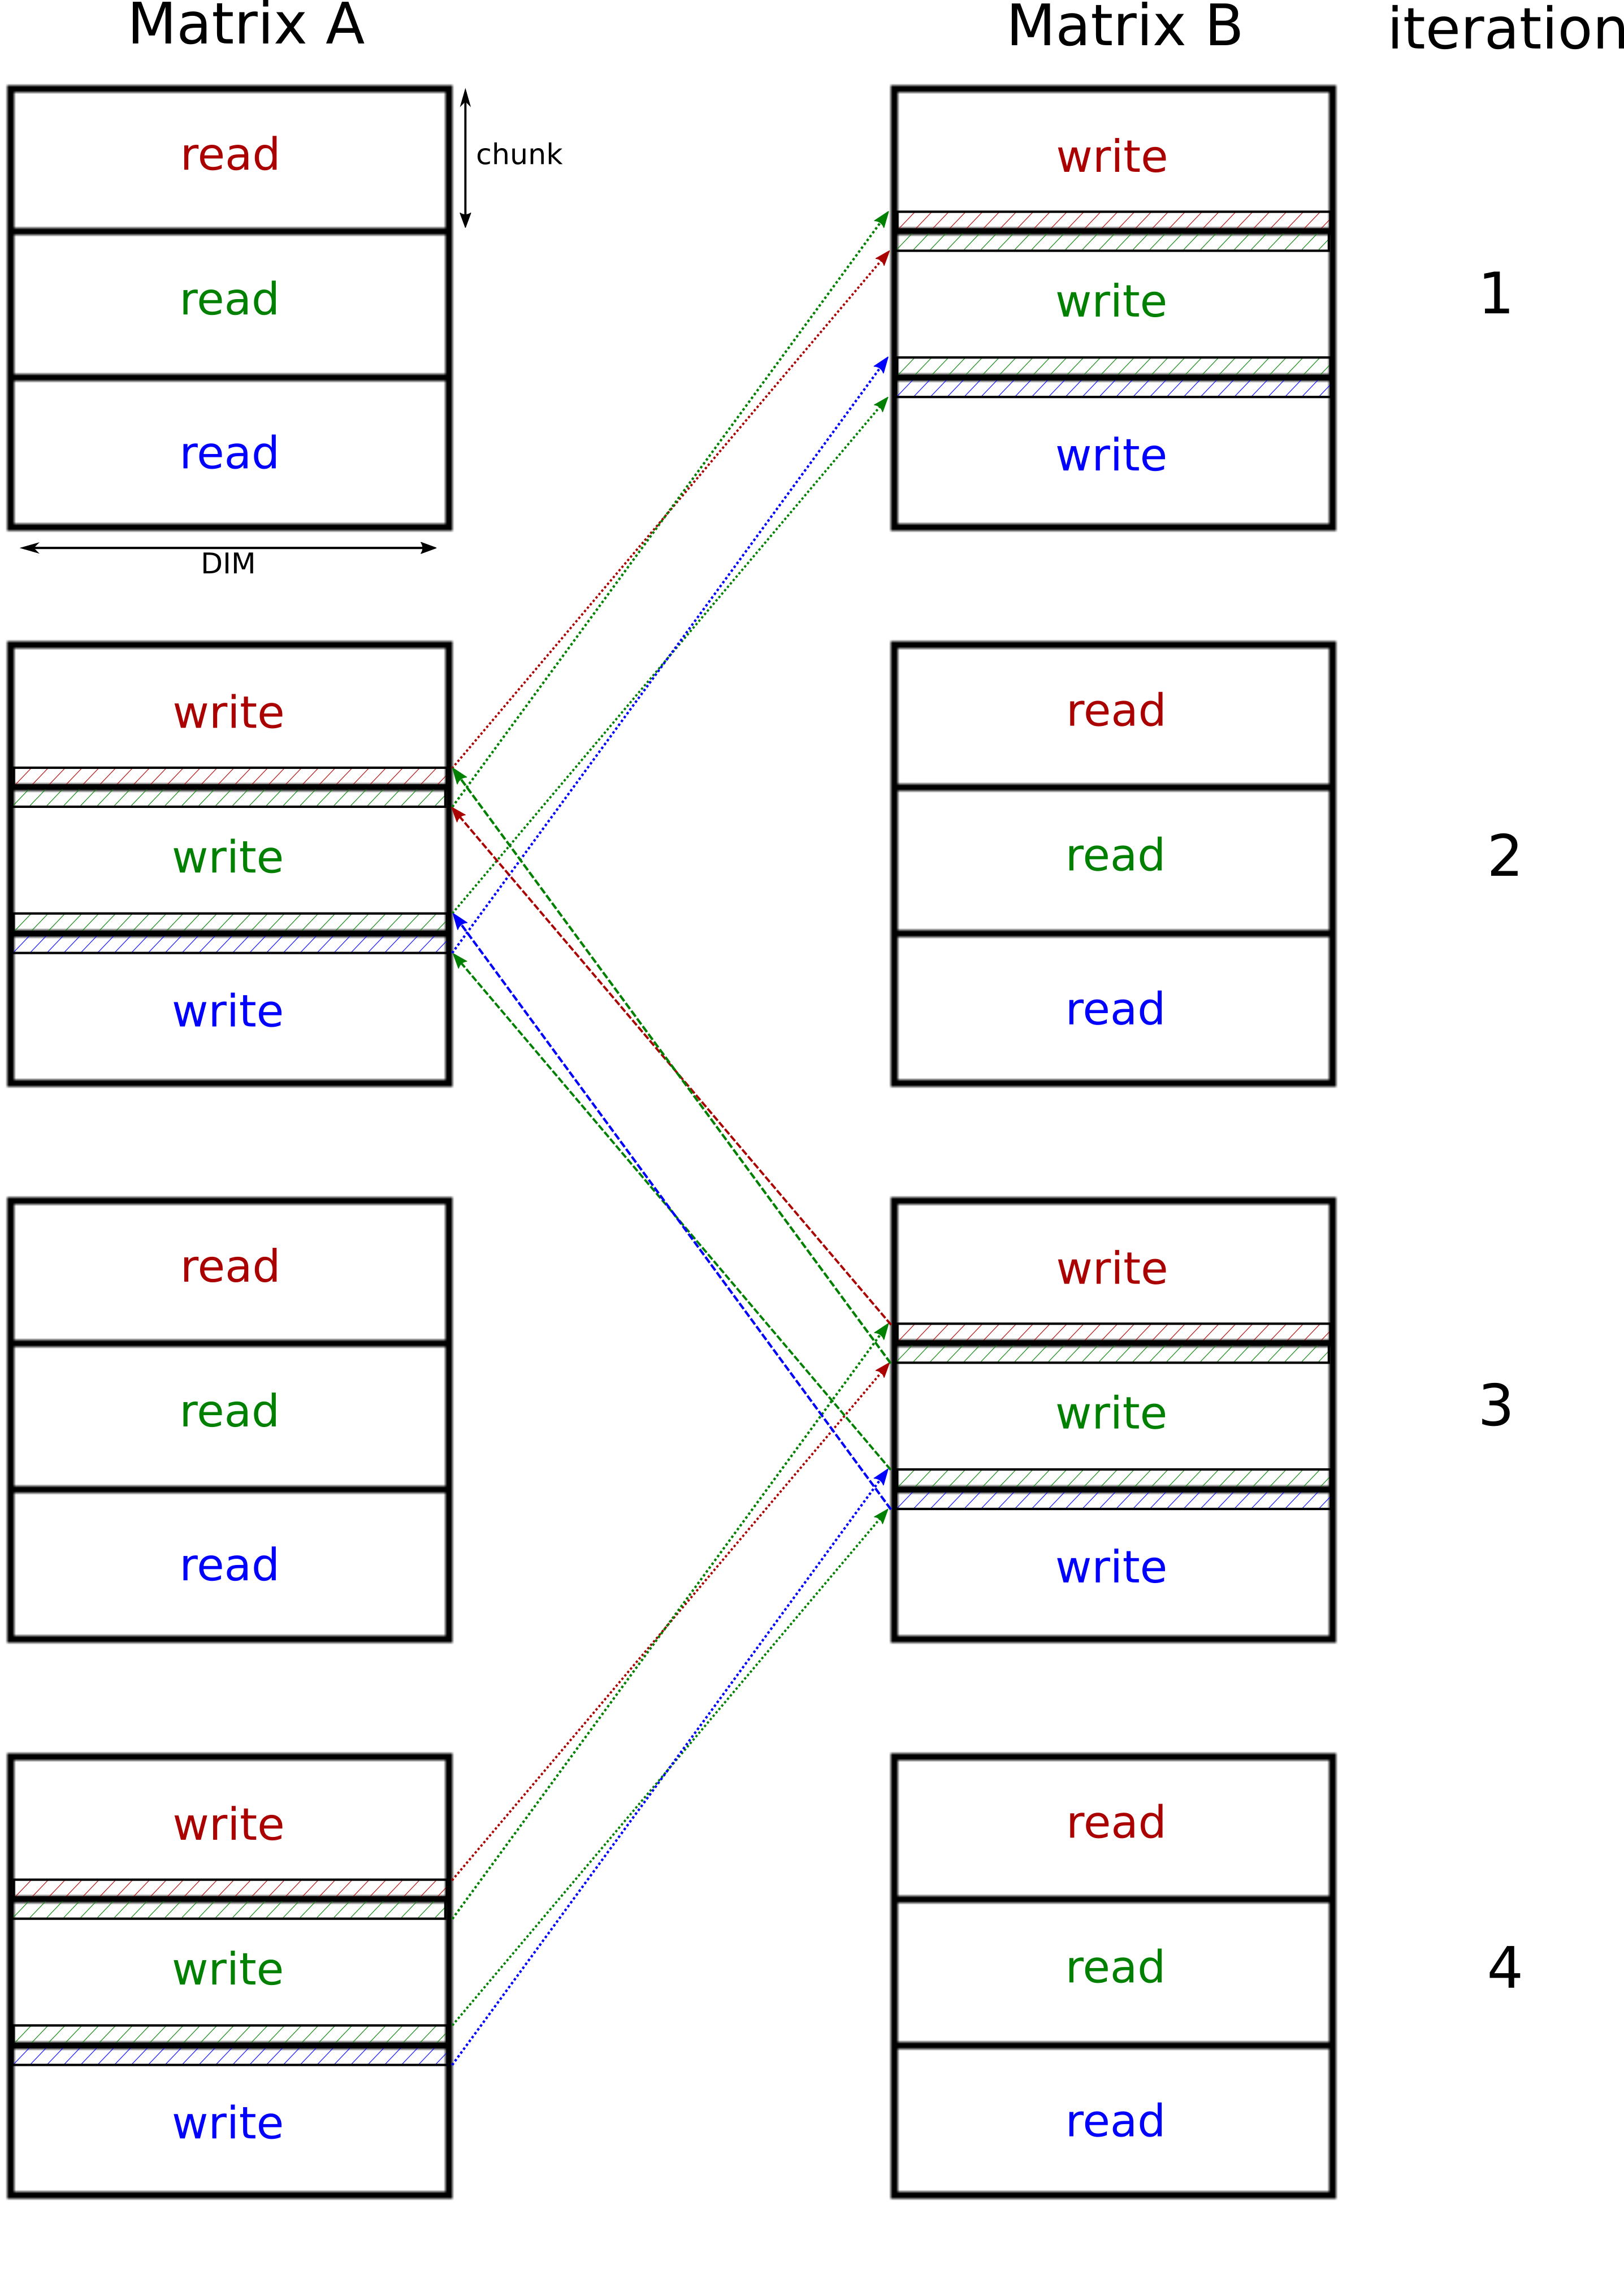
\includegraphics[width=10cm]{images/nowait.png}
  }
  \caption{Méthode \texttt{compute\_omp\_swap\_nowait}~: Utilisation
    de sémaphore pour retirer les barrières de synchronisation à
    chaque étape. L'exemple montre 3 threads qui effectuent 4
    itérations de l'algorithme. Chaque thread traite $chunk$ lignes de
    la matrice. Après chaque itération, on échange la matrice de
    lecture et d'écriture.}
  \label{fig:nowait}
\end{figure}

Pour implémenter ces dépendances, nous utilisons un tableau de
sémaphores de taille le nombre de dépendances soit $2*(nthreads-1)$,
et initialisées à 0. Chaque thread $t$ (excepté le dernier thread)
tente de décrémenter la sémaphore du thread $t+1$ avant d'écrire la
dernière ligne qui lui est attribuée, la ligne frontière entre deux
threads. De son côté, le thread $t+1$ incrémente la sémaphore
lorsqu'il a terminé de traiter la première ligne qui lui est
attribuée.
\medskip

On espère en pratique que les threads travaillent à la même vitesse
et que la sémaphore contient toujours la valeur 1.
\medskip

Lorsqu'un thread a stabilisé sa partie de la matrice, cela ne veut pas
dire qu'elle va rester stable, jusqu'à la fin. Les éboulement peuvent
ne pas encore être parvenu à ses frontières comme cela peut être le
cas lorsqu'on initialise une seule case à 100000. Ainsi, chaque thread
ayant stabilisé sa matrice s'endort sur une condition (une autre
sémaphore).
\medskip

Le dernier thread à avoir stabilisé sa matrice, plutôt que de
s'endormir lui aussi, réveille tous les autres en leur demandant
d'effectuer une dernière itération. Cette itération doit permettre de
savoir si des nouvelles valeurs ont été placées aux frontières pendant
qu'on était endormi. Si c'est le cas, on recommence le processus
depuis le départ. Sinon, l'algorithme se termine.
\medskip

Il est très important pour cette méthode que le nombre de threads soit
multiple de $DIM-2$ pour réduire au maximum le nombre de dépendances
et donc de prises de sémaphores.
\medskip

Pour éviter les inter-blocages, il faut aussi veiller à ne pas
s'endormir sur la sémaphore du thread voisin si celui-ci a stabilisé
son morceau de matrice et qu'il est endormi ou s'apprête à s'endormir.
\medskip

\subsubsection{Version OpenCL}

%%  LocalWords:  TODO chunk vector d'OpenMP omp nthreads p-itération
%%  LocalWords:  nowait OpenCL
